\documentclass[border=3pt, tikz]{standalone}
\usepackage[]{xcolor}
\usepackage[T1]{fontenc}
\usepackage{tikz, amsmath, pgfplots, longtable, relsize}
\usepackage[straightlabels, american, cuteinductors]{circuitikz}
\usetikzlibrary{arrows, shapes, pgfplots.groupplots, shapes.geometric}
\usetikzlibrary{patterns,calc, angles, quotes, decorations.markings, decorations, decorations.pathmorphing, decorations.shapes, patterns.meta}
\usepackage[normalem]{ulem}


\tikzset{arrow inside/.style = {postaction=decorate,decoration={markings,mark=at position 0.52 with \arrow{stealth}}}}

%%%%%%%%%% SET LOGIC GATE TYPE IN CIRCUITIKZ %%%%%%%%%%
\ctikzset{logic ports=ieee}
\newcommand{\textoverline}[1]{$\overline{\mbox{#1}}$}
\newcommand{\smaArrow}{{Latex[length=1mm]}}
\newcommand{\figArrow}{{Latex[length=2mm]}}
\newcommand{\flowBlock}{\node[draw, minimum width=3cm, minimum height=1cm, align=center]}
\newcommand{\flowDiamond}{\node[draw, minimum width=3cm, minimum height=1cm, align=center, diamond, aspect=1.5]}
\newcommand{\flowArrow}{\draw[-{Latex[length=2mm]}]}
\newcommand{\theArrow}{Latex[length=2mm]}
\newcommand{\medArrow}{Latex[length=4mm]}
\newcommand{\bigArrow}{{Latex[length=5mm]}}

\definecolor{sand}{RGB}{194, 178, 128}
\definecolor{ocean}{RGB}{79, 140, 207}


\def\checkmark{\tikz\fill[scale=0.4](0,.35) -- (.25,0) -- (1,.7) -- (.25,.15) -- cycle;}

%%% BEGIN DOCUMENT



\begin{document}




%%%%%%%%	CHAPTER 2
%%%%%%%%	OIL DRIPS
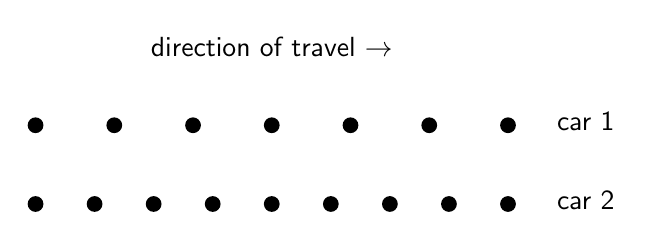
\begin{tikzpicture}[font=\sffamily]
	\def\R{0.1}
	
	\node[align=center] at (3,1) {direction of travel $\rightarrow$};
	
	\foreach \x in {0,...,6}	{
		\fill[black]	(\x,0) circle (\R);
	}
	\node[anchor=west, align=left] at (6.5,0.5*\R) {car 1};
	
	\foreach \x in {0,...,8}	{
		\fill[black]	(0.75*\x,-1) circle (\R);
	}
	\node[anchor=west, align=left] at (6.5,0.5*\R-1) {car 2};
\end{tikzpicture}




%%%%%%%%	CHAPTER 2
%%%%%%%%	BLOCKS AND PULLEY
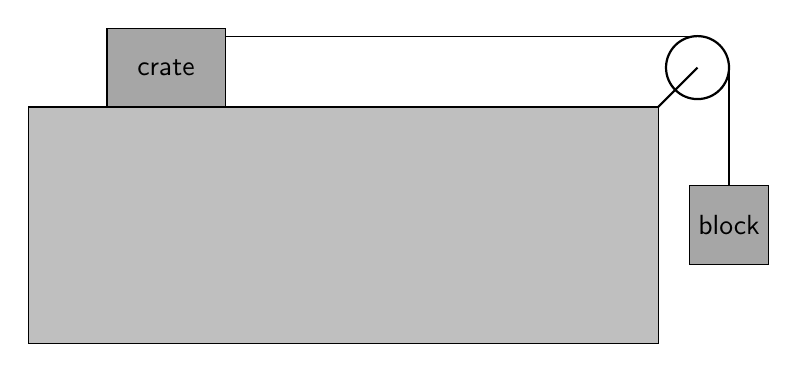
\begin{tikzpicture}[font=\sffamily]
	\fill[gray!50!white, draw=black]		(0,0) rectangle (8,-3);
	\draw[thick]					(8,0) --++ (0.5,0.5);
	\draw[thick]					(8.5,0.5) circle (0.4);
	\fill[gray!70!white, draw=black]		(1,0) rectangle (2.5,1) node[midway, text=black] {crate};
	\draw[]						(2.5,0.9) --++ (right:6);
	\draw[]						(8.9,0.5) --++ (down:1.5);
	\fill[gray!70!white, draw=black]		(8.4,-1) rectangle (9.4,-2) node[midway, text=black] {block};
\end{tikzpicture}



%%%%%%%%	CHAPTER 2
%%%%%%%%	PATH AND DISPLACEMENT
\begin{tikzpicture}[font=\sffamily]
	\def\L{0.3}
	\draw[thick]	(-7,0) -- (7,0);
	\foreach \x in {-7,...,7} {
		\draw[]	(\x,-0.5*\L) node[below, anchor=north, align=center] {\x} --++ (up:\L);
	}
	\node[align=center, anchor=north] at (0,-1) {position (m)};
	
	\node[inner sep=0pt, opacity=0.5] at (0,1.1)	{\includegraphics[height=2.2 cm]{fig/standing.png}};
	\draw[line width=3pt, -\bigArrow]	(0,2.5) --++ (right:3);
	\node[inner sep=0pt, opacity=1] at (2.5,1)		{\includegraphics[height=2.5 cm]{fig/running.png}};
\end{tikzpicture}

\begin{tikzpicture}[font=\sffamily]
	\def\L{0.3}
	\draw[thick]	(-7,0) -- (7,0);
	\foreach \x in {-7,...,7} {
		\draw[]	(\x,-0.5*\L) node[below, anchor=north, align=center] {\x} --++ (up:\L);
	}
	\node[align=center, anchor=north] at (0,-1) {position (m)};
	
	\node[inner sep=0pt, opacity=1, xscale=-1] at (2.5,1)		{\includegraphics[height=2.5 cm]{fig/running.png}};
	\draw[line width=3pt, -\bigArrow]	(1.5,1) --++ (left:2.5);
\end{tikzpicture}





%%%%%%%%	CHAPTER 2
%%%%%%%%	STATIC EQUILIBRIUM
\begin{tikzpicture}[font=\sffamily]
	\tikzset	{
		scale/.pic={
			code={       
				\draw[]		(0,0) circle (0.4);
				\draw[line width=1.5pt, -\figArrow]		(0,0) --++ (up:0.35);
				\draw[]		(-0.5,0.4) --++ (right:1) --++ (down:0.7) --++ (-0.2,-0.2) --++ (left:0.6) --++ (-0.2,0.2) -- cycle;
				\draw[]		(-0.2,0.4) rectangle (0.2,0.5);
				\fill[gray!70!white, draw=black]	(-0.5,0.5) rectangle (0.5,0.6);
				\draw[]		(-0.5,-0.6) rectangle (0.5,-0.5);
			}
		},
	}
        \pic[] at (-5,0) {scale};
        \pic[] at (5,0) {scale};
	\node[inner sep=0pt] at (0,2.05)	{\includegraphics[height=2.5 cm]{fig/standing.png}};
	\draw[]	(-6,0.6) rectangle (6,0.8);
\end{tikzpicture}

\begin{tikzpicture}[font=\sffamily]
	\tikzset	{
		scale/.pic={
			code={       
				\draw[]		(0,0) circle (0.4);
				\draw[line width=1.5pt, -\figArrow]		(0,0) --++ (up:0.35);
				\draw[]		(-0.5,0.4) --++ (right:1) --++ (down:0.7) --++ (-0.2,-0.2) --++ (left:0.6) --++ (-0.2,0.2) -- cycle;
				\draw[]		(-0.2,0.4) rectangle (0.2,0.5);
				\fill[gray!70!white, draw=black]	(-0.5,0.5) rectangle (0.5,0.6);
				\draw[]		(-0.5,-0.6) rectangle (0.5,-0.5);
			}
		},
	}
        \pic[] at (-5,0) {scale};
        \pic[] at (5,0) {scale};
	\node[inner sep=0pt] at (2,2.05)	{\includegraphics[height=2.5 cm]{fig/standing.png}};
	\draw[]	(-6,0.6) rectangle (6,0.8);
\end{tikzpicture}

\begin{tikzpicture}[font=\sffamily]
	\tikzset	{
		scale/.pic={
			code={       
				\draw[]		(0,0) circle (0.4);
				\draw[line width=1.5pt, -\figArrow]		(0,0) --++ (up:0.35);
				\draw[]		(-0.5,0.4) --++ (right:1) --++ (down:0.7) --++ (-0.2,-0.2) --++ (left:0.6) --++ (-0.2,0.2) -- cycle;
				\draw[]		(-0.2,0.4) rectangle (0.2,0.5);
				\fill[gray!70!white, draw=black]	(-0.5,0.5) rectangle (0.5,0.6);
				\draw[]		(-0.5,-0.6) rectangle (0.5,-0.5);
			}
		},
	}
        \pic[] at (-5,0) {scale};
        \pic[] at (5,0) {scale};
	\node[inner sep=0pt] at (0,2.05)	{\includegraphics[height=2.5 cm]{fig/standing.png}};
	\node[inner sep=0pt] at (2,2.05)	{\includegraphics[height=2.5 cm]{fig/standing.png}};
	\draw[]	(-6,0.6) rectangle (6,0.8);
\end{tikzpicture}






%%%%%%%%	CHAPTER 3
%%%%%%%%	NEWTON'S THIRD LAW
\begin{tikzpicture}[font=\sffamily]
	\def\H{0.25}
	\def\W{0.25}
	\def\X{-3.25}
	
	\fill[gray!50!white, draw=black]		(-4,-\H) rectangle (4,0);
	\fill[gray!50!white, draw=black]		(-3-\W,-2) rectangle (-3,-\H);
	\fill[gray!50!white, draw=black]		(3+\W,-2) rectangle (3,-\H);

	\draw[thick]		(-5,-2) --++ (right:10);
	\fill[gray!30!white]	(-5,-2) rectangle (5,-3); 

	\node[inner sep=0pt] at (0,1.25)	{\includegraphics[height=2.5 cm]{fig/standing.png}};

	\foreach \name/\init/\y in {person/P/1.25, table/T/-1, Earth/E/-2.5} {
		\node[align=right, anchor=east] at (\X,\y)	{\name~(\init)};
	}
	
	\foreach \inits/\y/\dir in {PE/1.75/down, PT/0/up, TP/-0.25/down, EP/-2/up} {
		\draw[line width=4pt, -\medArrow]	(1,\y) --++ (\dir:0.8) node[midway, right, anchor=west] {F\textsubscript{\inits}};
	}

\end{tikzpicture}






%%%%%%%%	CHAPTER 3
%%%%%%%%	AIRPLANE
\begin{tikzpicture}[font=\sffamily]
	\node[inner sep=0pt] at (0,0)	{\includegraphics[width=5 cm]{fig/airplane.png}};

	\foreach \x in {-5,...,5} {
		\draw[line width=1.5pt, -\figArrow]	(\x,5) --++ (down:2);
	}
	
	\node[align=center, anchor=south] at (0,5) {steady headwind};
\end{tikzpicture}

\begin{tikzpicture}[font=\sffamily]
	\node[inner sep=0pt] at (0,0)	{\includegraphics[width=5 cm]{fig/airplane.png}};

	\foreach \x in {-5,...,5} {
		\draw[line width=1.5pt, -\figArrow]	(\x,-5) --++ (up:2);
	}
	
	\node[align=center, anchor=north] at (0,-5) {steady tailwind};
\end{tikzpicture}

\begin{tikzpicture}[font=\sffamily]
	\node[inner sep=0pt] at (0,0)	{\includegraphics[width=5 cm]{fig/airplane.png}};

	\foreach \y in {-4,...,4} {
		\draw[line width=1.5pt, -\figArrow]	(-5,\y) --++ (right:2);
	}
	
	\node[align=center, anchor=south, rotate=90] at (-5,0) {steady crosswind};
\end{tikzpicture}







%%%%%%%%	CHAPTER 4
%%%%%%%%	2D COLLISION
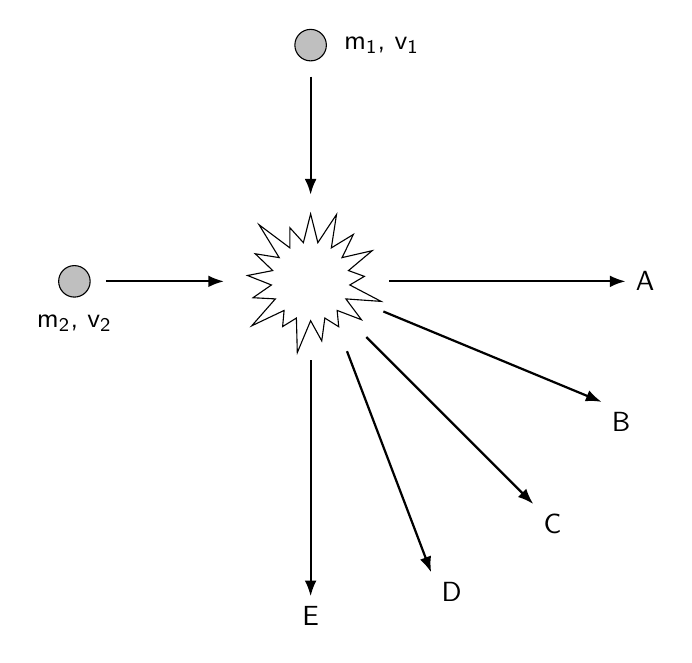
\begin{tikzpicture}[font=\sffamily]
	\def\R{0.2}
	
	\coordinate (O) at (0,0);
	\coordinate (A) at (4,0);
	\coordinate (B) at (3.696,-1.531);
	\coordinate (C) at (2.828,-2.828);
	\coordinate (D) at (1.531,-3.696);
	\coordinate (E) at (0,-4);
	\coordinate (M1) at (0,3);
	\coordinate (M2) at (-3,0);
	
	\foreach \name/\ang/\anchor in {A/0/right, B/-22.5/below right, C/-45/below right, D/-62.5/below right, E/-90/below} {
		\draw[thick, -\figArrow]	(\ang:1) -- (\name) node[\anchor] {\name};
	}
	
	\fill[gray!50!white, draw=black]		(M1) circle (\R);
		\node[anchor=west, align=left] at	($(M1)+(1.5*\R,0)$) {m\textsubscript{1}, v\textsubscript{1}};
		\draw[thick, -\figArrow]			($(M1)+(0,-2*\R)$) --++ (down:1.5);
	\fill[gray!50!white, draw=black]		(M2) circle (\R);
		\node[anchor=north, align=center] at	($(M2)+(0,-1.5*\R)$) {m\textsubscript{2}, v\textsubscript{2}};
		\draw[thick, -\figArrow]			($(M2)+(2*\R,0)$) --++ (right:1.5);

	\node[starburst, draw, minimum width=2cm, minimum height=2cm] at (O) {};

\end{tikzpicture}






%%%%%%%%	CHAPTER 4
%%%%%%%%	SIMPLE MACHINES
\begin{tikzpicture}[font=\sffamily]
	\def\W{2}
	\def\bw{0.85}
	\def\bh{1}
	\def\H{2.5}
	\def\off{1.5}
	
	\node[inner sep=0pt] at (0,0.5*\H)	{\includegraphics[height=\H cm]{fig/arms-up}};
	\draw[]	(-\W,0) -- (\W,0);
	\fill[pattern=north east lines]	(-\W,0) rectangle (\W,-0.25);
	
	\fill[gray!50!white, draw=black]	(-\bw,\H) rectangle (\bw,\H+\bh);
	
	\draw[thick, \figArrow-\figArrow]	(\off,0) --++ (up:\H) node[midway, fill=white, align=center] {H};
\end{tikzpicture}
% RAMP
\begin{tikzpicture}[font=\sffamily]
	\def\W{3.5}
	\def\bw{0.85}
	\def\bh{1}
	\def\H{1.5}
	\def\off{-3}
	
	\node[inner sep=0pt] at (2.82,0.5*\H)	{\includegraphics[height=\H cm]{fig/push.png}};
	\draw[]	(-\W,0) -- (\W,0);
	\fill[pattern=north east lines]	(-\W,0) rectangle (\W,-0.25);
	
	\fill[gray!50!white, draw=black, rotate=-23.2]	(-0.25,1) rectangle (-0.25+2*\bw,1+\bh);
	
	\fill[gray!80!white, draw=black] (-2.5,0) --++ (up:\H) --++ (right:2) -- (3,0) -- cycle;
	
	\draw[thick, \figArrow-\figArrow]	(\off,0) --++ (up:\H) node[midway, fill=white, align=center] {H};
\end{tikzpicture}
% PULLEY
\begin{tikzpicture}[font=\sffamily]
	\def\W{2.5}
	\def\P{1}
	\def\pw{0.1}
	\def\bw{0.85}
	\def\bh{1}
	\def\H{1.5}
	\def\off{-2}
	\def\Pa{1.25*\H}
	\def\Pb{2*\H}
	\def\Pc{2.35*\H}
	\def\R{0.2}
	\def\Rb{0.25}
	\coordinate (arm) at (1.08,0.93);
	
	%person
	\node[inner sep=0pt] at (1.5,0.5*\H)	{\includegraphics[height=\H cm]{fig/arm-out}};
	
	%ground
	\draw[]	(-\W,0) -- (\W,0);
	\fill[pattern=north east lines]	(-\W,0) rectangle (\W,-0.25);

	\draw[]	(-\P,\H+2.5) -- (\P,\H+2.5);
	\fill[pattern=north east lines]	(-\P,\H+2.5) rectangle (\P,\H+2.75);
	
	%pulley
	\fill[black]	(0,\Pa) circle (\Rb);
	\fill[black]	(0,\Pb) circle (\R);
	\fill[black]	(0,\Pc) circle (\Rb);
	\fill[white, draw=black]	(-0.5*\pw,\H+2.5) rectangle (0.5*\pw,\Pb-1.5*\R);
	\fill[white, draw=black]	(-0.5*\pw,\bh+0.5) rectangle (0.5*\pw,\Pa+1.5*\R);
	\draw[thick]			(0,\bh) --++ (up:0.5);
	
	%rope
	\draw[thick]	(arm) -- (0.96*\Rb,\Pc);
	\draw[thick]	(-0.95*\Rb,\Pc) -- (-0.95*\Rb,\Pa);
	\draw[thick]	(0.95*\Rb,\Pa) -- (0.95*\R,\Pb);
	\draw[thick]	(-0.95*\R,\Pb) -- (0,\Pa+1.5*\R);
	
	%box
	\fill[gray!50!white, draw=black]	(-\bw,0.25) rectangle (\bw,0.25+\bh);
	
	\draw[thick, \figArrow-\figArrow]	(\off,0) --++ (up:\H) node[midway, fill=white, align=center] {H};
\end{tikzpicture}






%%%%%%%%	CHAPTER 4
%%%%%%%%	TWO FISH
\begin{tikzpicture}[font=\sffamily]
	% big fish
	\def\B{-4}	%x position
	\def\bh{1.5} %height of big fish
	% small fish
	\def\S{4}	%x position
	\def\bs{0.75} %height of big fish

	\node[inner sep=0pt, xscale=-1] at (\B,0)	{\includegraphics[height=\bh cm]{fig/fish}};
	\node[inner sep=0pt] at (\S,0)			{\includegraphics[height=\bs cm]{fig/fish}};

	\draw[thick, -\figArrow]	(\B,1.5) --++ (right:2.5) node[right] {v\textsubscript{large}};
	\draw[thick, -\figArrow]	(\S,1.5) --++ (left:2.5) node[left] {v\textsubscript{small}};
\end{tikzpicture}





%%%%%%%%	CHAPTER 4
%%%%%%%%	VERTICAL TOSS
\begin{tikzpicture}[font=\sffamily]
	\def\W{2}
	\def\bh{3.5}
	\def\R{0.1}
	\def\H{2.5}
	
	%platform
	\fill[gray!50!white, draw=black]	(-\W,\H) rectangle (0,0);
	\draw[thick, \figArrow-\figArrow]	(-0.5*\W,0) --++ (up:\H) node[midway, fill=gray!50!white, align=center] {H};

	%person
	\node[inner sep=0pt] at (-0.25*\W,1.5*\H)	{\includegraphics[height=\H cm]{fig/arms-up}};
	
	%floor
	\draw[]	(-\W,0) -- (\W,0);
	\fill[pattern=north east lines]	(-\W,0) rectangle (\W,-0.25);
	
	%ball
	\fill[gray!80!white, draw=black]	(0.5*\W, \H+\bh) circle (\R);
	\draw[thick, \figArrow-\figArrow]	(0.7*\W,\H) --++ (up:\bh) node[midway, fill=white, align=center] {h};
	
\end{tikzpicture}





%%%%%%%%	CHAPTER 5
%%%%%%%%	TORQUE
\begin{tikzpicture}[font=\sffamily]
	\def\H{5}
	\def\W{5}
	\def\R{0.05}
	\coordinate (A) at (0,-0.5*\H);
	\coordinate (B) at (0,-0.325*\H);
	\coordinate (C) at (0,-0.15*\H);
	\coordinate (D) at (0,0.025*\H);
	\coordinate (F1) at (0.175*\W, 0.5*\H);
	\coordinate (F2) at (0, 0.5*\H);
	\coordinate (F3) at (-0.5*\W, -0.2*\H);
	\coordinate (F4) at (0.175*\W, -0.2*\H);
	
	\draw[]		(-0.5*\W,-0.5*\H) --++ (up:0.3*\H) --++ (right:0.3*\W) --++ (up:0.7*\H) --++ (right:0.35*\W) --++ (down:0.7*\H) --++ (right:0.3*\W) --++ (down:0.3*\H) -- cycle;
	
	\foreach \name in {A, B, C, D} {
		\fill[black]	(\name) circle (\R) node[above left] {\name};
	}
	
	\foreach \num/\x/\y/\pos in {1/1.5/0/right, 2/0/1.5/above, 3/-1.5/0/left, 4/1.06/1.06/above right} {
		\draw[dashed, -\figArrow]	(F\num) --++ (\x,\y) node[\pos] {F\textsubscript{\num}};
	}
	
\end{tikzpicture}






%%%%%%%%	CHAPTER 5
%%%%%%%%	ORBITS
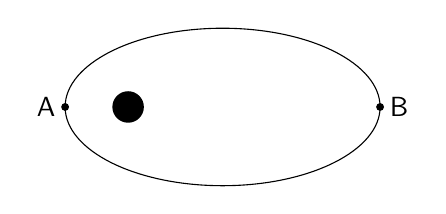
\begin{tikzpicture}[font=\sffamily]
	\def\maj{2}
	\def\min{1}
	\def\R{0.2}
	\def\p{0.05}
	\coordinate (A) at (-\maj,0);
	\coordinate (B) at (\maj,0);
	\coordinate (F) at (-0.6*\maj,0);

	\draw[]	(0,0) circle [x radius=\maj, y radius=\min];	
	\fill[black]	(A) circle (\p) node[left] {A};
	\fill[black]	(B) circle (\p) node[right] {B};
	\fill[black]	(F) circle (\R);
\end{tikzpicture}








%%%%%%%%	CHAPTER 5
%%%%%%%%	ORBITS 2
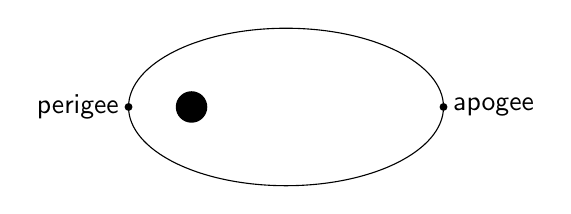
\begin{tikzpicture}[font=\sffamily]
	\def\maj{2}
	\def\min{1}
	\def\R{0.2}
	\def\p{0.05}
	\coordinate (A) at (-\maj,0);
	\coordinate (B) at (\maj,0);
	\coordinate (F) at (-0.6*\maj,0);

	\draw[]	(0,0) circle [x radius=\maj, y radius=\min];	
	\fill[black]	(A) circle (\p) node[left] {perigee};
	\fill[black]	(B) circle (\p) node[right] {apogee};
	\fill[black]	(F) circle (\R);
\end{tikzpicture}





%%%%%%%%	CHAPTER 5
%%%%%%%%	SPINNING WHEELS
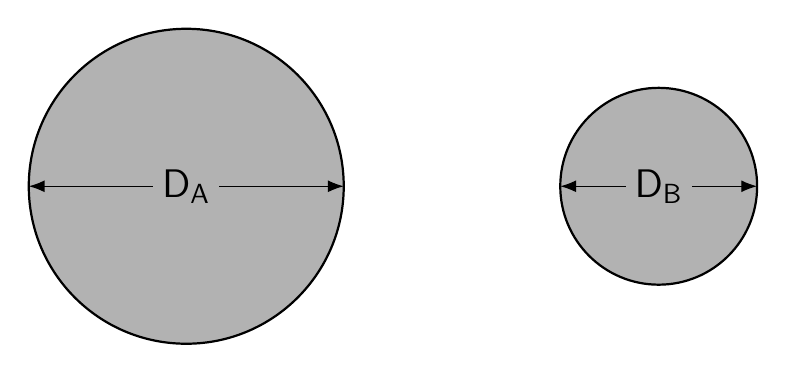
\begin{tikzpicture}[font=\sffamily\Large]
	\coordinate (A) at (-3,0);
	\def\Ra{2}
	\coordinate (B) at (3,0);
	\def\Rb{1.25}
	
	\fill[gray!60!white, draw=black, thick]	(A) circle (\Ra);
		\draw[\figArrow-\figArrow]	($(A)-(\Ra,0)$) --++ (right:2*\Ra) node[midway, fill=gray!60!white] {D\textsubscript{A}};
	\fill[gray!60!white, draw=black, thick]	(B) circle (\Rb);
		\draw[\figArrow-\figArrow]	($(B)-(\Rb,0)$) --++ (right:2*\Rb) node[midway, fill=gray!60!white] {D\textsubscript{B}};

\end{tikzpicture}

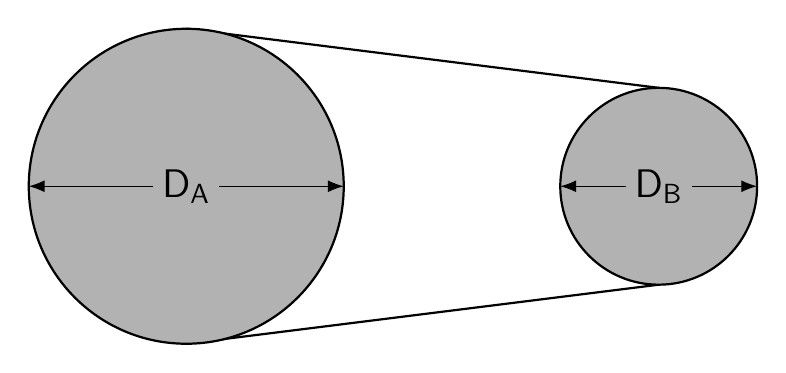
\begin{tikzpicture}[font=\sffamily\Large]
	\coordinate (A) at (-3,0);
	\def\Ra{2}
	\coordinate (B) at (3,0);
	\def\Rb{1.25}

	\draw[thick]	($(A)+(0,\Ra)$) -- ($(B)+(0,\Rb)$);
	\draw[thick]	($(A)+(0,-\Ra)$) -- ($(B)+(0,-\Rb)$);
	
	\fill[gray!60!white, draw=black, thick]	(A) circle (\Ra);
		\draw[\figArrow-\figArrow]	($(A)-(\Ra,0)$) --++ (right:2*\Ra) node[midway, fill=gray!60!white] {D\textsubscript{A}};
	\fill[gray!60!white, draw=black, thick]	(B) circle (\Rb);
		\draw[\figArrow-\figArrow]	($(B)-(\Rb,0)$) --++ (right:2*\Rb) node[midway, fill=gray!60!white] {D\textsubscript{B}};
\end{tikzpicture}










%%%%%%%%	CHAPTER 5
%%%%%%%%	STALLED TRUCK
\begin{tikzpicture}[font=\sffamily]
	\def\W{10}
	\def\H{0.75}
	\def\pylon{0.5}
	\coordinate (L) at (-0.5*\W,0);
	\coordinate (T) at (-2,0);
	\coordinate (R) at (0.5*\W,0);

	
	\draw[thick] decorate [decoration={random steps}]	{(L) --++ (3,-3)};
	\draw[thick] decorate [decoration={random steps}]	{(R) --++ (-3,-3)};
	\fill[gray!80!white, draw=black]	(L) rectangle ($(R)+(0,-0.25)$);
	\fill[gray!80!white, draw=black]	($(L)-(0,0.25)$) rectangle ($(L)+(\pylon,-\pylon-0.25)$);
	\fill[gray!80!white, draw=black]	($(R)-(0,0.25)$) rectangle ($(R)-(\pylon,\pylon+0.25)$);
	\draw[thick]	($(L)-(1.5,0)$) -- ($(R)+(1.5,0)$);
	
	\node[inner sep=0pt] at ($(T)+(0,0.5*\H)$)	{\includegraphics[height=\H cm]{fig/truck}};

	\draw[thick,-\figArrow]	($(L)+(0.5*\pylon,0)$) --++ (up:2) node[above] {F\textsubscript{left}};
	\draw[thick,-\figArrow]	($(R)-(0.5*\pylon,0)$) --++ (up:1.5) node[above] {F\textsubscript{right}};
	\draw[thick,-\figArrow]	($(T)+(0,0.5*\H)$) --++ (down:2) node[below] {weight};
\end{tikzpicture}








%%%%%%%%	CHAPTER 6
%%%%%%%%	SPRINGS
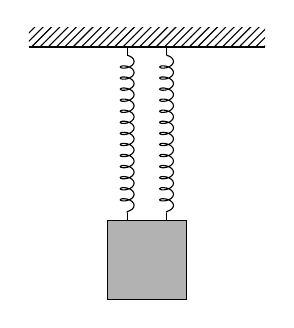
\begin{tikzpicture}[font=\sffamily]
	\def\W{1.5}
	\def\off{0.1}
	\def\H{2}
	\def\S{0.5}
	\def\B{1}

	\fill[pattern=north east lines]	(-\W,\H) rectangle (\W,\H+0.25);
	\draw[thick]				(-\W,\H) -- (\W,\H);
	
	\draw[]	(-0.5*\S,\H) --++ (down:\off);
	\draw[]	(0.5*\S,\H) --++ (down:\off);
	\draw[decorate,decoration={coil,segment length=4pt}]	(-0.5*\S,\H-\off) --++ (down:2);
	\draw[decorate,decoration={coil,segment length=4pt}]	(0.5*\S,\H-\off) --++ (down:2);
	\draw[]	(-0.5*\S,\H-\off-2) --++ (down:\off);
	\draw[]	(0.5*\S,\H-\off-2) --++ (down:\off);
	
	\fill[gray!60!white, draw=black]	(-0.5*\B,\H-2*\off-2) rectangle ++(\B,-\B);
\end{tikzpicture}
%series
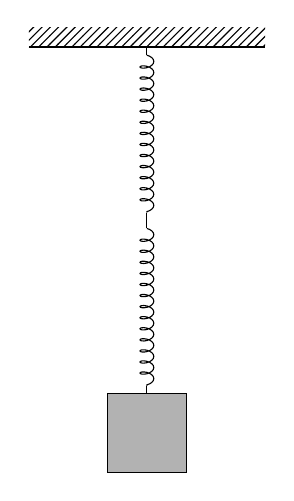
\begin{tikzpicture}[font=\sffamily]
	\def\W{1.5}
	\def\off{0.1}
	\def\H{2}
	\def\S{0.5}
	\def\B{1}

	\fill[pattern=north east lines]	(-\W,\H) rectangle (\W,\H+0.25);
	\draw[thick]				(-\W,\H) -- (\W,\H);
	
	\draw[]	(0,\H) --++ (down:\off);
	\draw[decorate,decoration={coil,segment length=4pt}]	(0,\H-\off) --++ (down:2);
	\draw[]	(0,\H-\off-2) --++ (down:2*\off);
	\draw[decorate,decoration={coil,segment length=4pt}]	(0,\H-2-3*\off) --++ (down:2);
	\draw[]	(0,\H-4-3*\off) --++ (down:\off);
	
	\fill[gray!60!white, draw=black]	(-0.5*\B,\H-4*\off-4) rectangle ++(\B,-\B);
\end{tikzpicture}
%series + parallel
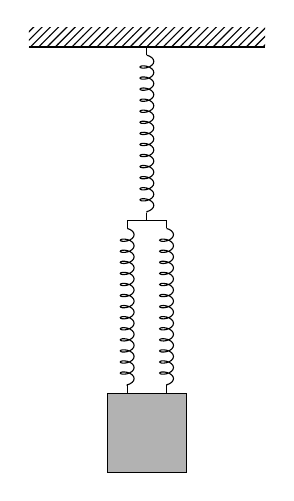
\begin{tikzpicture}[font=\sffamily]
	\def\W{1.5}
	\def\off{0.1}
	\def\H{2}
	\def\S{0.5}
	\def\B{1}

	\fill[pattern=north east lines]	(-\W,\H) rectangle (\W,\H+0.25);
	\draw[thick]				(-\W,\H) -- (\W,\H);
	
	\draw[]	(0,\H) --++ (down:\off);
	\draw[decorate,decoration={coil,segment length=4pt}]	(0,\H-\off) --++ (down:2);
	\draw[]	(0,\H-\off-2) --++ (down:\off);

	\draw[]	(-0.5*\S,\H-2-2*\off) --++ (right:\S);
	\draw[]	(-0.5*\S,\H-2-2*\off) --++ (down:\off);
	\draw[]	(0.5*\S,\H-2-2*\off) --++ (down:\off);
	\draw[decorate,decoration={coil,segment length=4pt}]	(-0.5*\S,\H-2-3*\off) --++ (down:2);
	\draw[decorate,decoration={coil,segment length=4pt}]	(0.5*\S,\H-2-3*\off) --++ (down:2);
	\draw[]	(-0.5*\S,\H-3*\off-4) --++ (down:\off);
	\draw[]	(0.5*\S,\H-3*\off-4) --++ (down:\off);
	
	\fill[gray!60!white, draw=black]	(-0.5*\B,\H-4*\off-4) rectangle ++(\B,-\B);
\end{tikzpicture}







%%%%%%%%	CHAPTER 7
%%%%%%%%	ARCHIMEDES PRINCIPLE
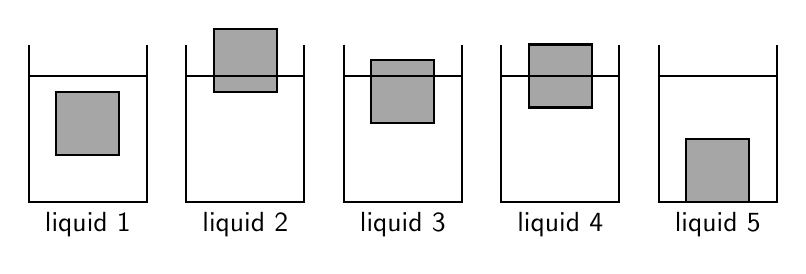
\begin{tikzpicture}[font=\sffamily]
	\def\off{2}
	\def\W{1.5}
	\def\H{2}
	\def\B{0.8}
	\coordinate (B1) at (0,-0.5*\H);
	\coordinate (B2) at (0,-0.1*\H);
	\coordinate (B3) at (0,-0.3*\H);
	\coordinate (B4) at (0,-0.2*\H);
	\coordinate (B5) at (0,-0.8*\H);
	
	\foreach \x in {1,...,5} {
		\draw[thick, fill=gray!70!white]	($(-0.5*\B,0.5*\B)+(B\x)+(\x*\off+0.5*\W,0)$) rectangle ++(\B,-\B);
		\draw[thick]	(0+\x*\off,0) --++ (down:\H) --++ (right:\W) --++ (up:\H);
		\draw[thick]	(0+\x*\off,-0.2*\H) --++ (right:\W);
		\node[anchor=north, align=center] at (\x*\off+0.5*\W,-\H) {liquid~\x};
	}
\end{tikzpicture}







%%%%%%%%	CHAPTER 7
%%%%%%%%	ENCLOSED GAS
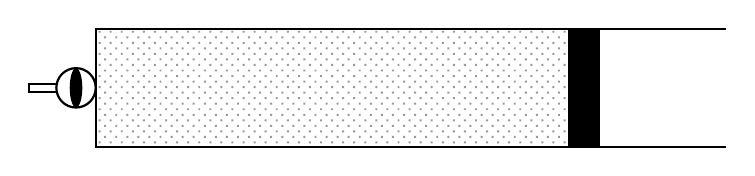
\begin{tikzpicture}[font=\sffamily]
	\def\plunger{6}
	\def\W{8}
	\def\H{1.5}
	\def\R{0.25}
	\def\Rm{0.08}
	\def\ht{0.1}

	\fill[pattern={Dots[angle=45,distance={4pt/sqrt(2)}]}, opacity=0.4]		(0,0.5*\H) rectangle (\plunger,-0.5*\H);
	\draw[thick]			(\W,0.5*\H) --++ (left:\W) --++ (down:\H) --++ (right:\W);	
	\fill[black]				(\plunger,0.5*\H) rectangle ++(0.4,-\H);
	\draw[thick]			(-\R,0.5*\ht) rectangle ++(-0.6,-\ht);
	\draw[thick, fill=white]	(-\R,0) circle (\R);
	\fill[black]				(-\R,0) circle [x radius=\Rm, y radius=\R];
\end{tikzpicture}
% compressed
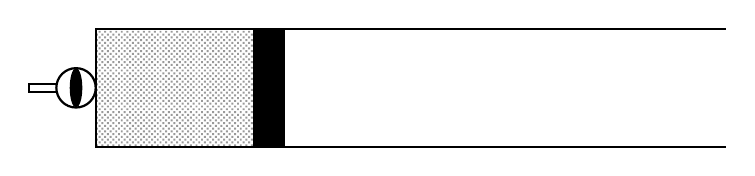
\begin{tikzpicture}[font=\sffamily]
	\def\plunger{2}
	\def\W{8}
	\def\H{1.5}
	\def\R{0.25}
	\def\Rm{0.08}
	\def\ht{0.1}

	\fill[pattern={Dots[angle=45,distance={2pt/sqrt(2)}]}, opacity=0.4]		(0,0.5*\H) rectangle (\plunger,-0.5*\H);
	\draw[thick]			(\W,0.5*\H) --++ (left:\W) --++ (down:\H) --++ (right:\W);	
	\fill[black]				(\plunger,0.5*\H) rectangle ++(0.4,-\H);
	\draw[thick]			(-\R,0.5*\ht) rectangle ++(-0.6,-\ht);
	\draw[thick, fill=white]	(-\R,0) circle (\R);
	\fill[black]				(-\R,0) circle [x radius=\Rm, y radius=\R];
\end{tikzpicture}
% let gas out
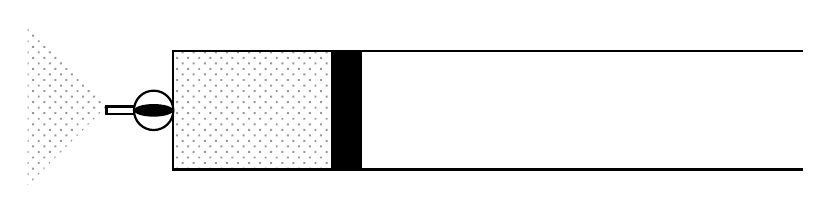
\begin{tikzpicture}[font=\sffamily]
	\def\plunger{2}
	\def\W{8}
	\def\H{1.5}
	\def\R{0.25}
	\def\Rm{0.08}
	\def\ht{0.1}

	\fill[pattern={Dots[angle=45,distance={4pt/sqrt(2)}]}, opacity=0.4]		(-\R-0.6,0.05) --++ (-1,1) --++ (down:2) -- cycle;


	\fill[pattern={Dots[angle=45,distance={4pt/sqrt(2)}]}, opacity=0.4]		(0,0.5*\H) rectangle (\plunger,-0.5*\H);
	\draw[thick]			(\W,0.5*\H) --++ (left:\W) --++ (down:\H) --++ (right:\W);	
	\fill[black]				(\plunger,0.5*\H) rectangle ++(0.4,-\H);
	\draw[thick]			(-\R,0.5*\ht) rectangle ++(-0.6,-\ht);
	\draw[thick, fill=white]	(-\R,0) circle (\R);
	\fill[black]				(-\R,0) circle [y radius=\Rm, x radius=\R];
\end{tikzpicture}
% expanded
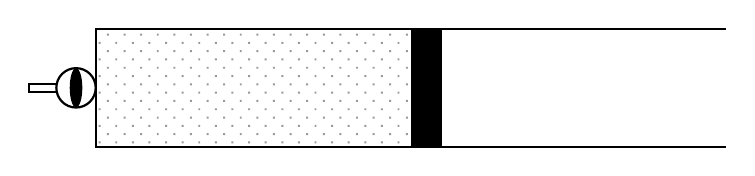
\begin{tikzpicture}[font=\sffamily]
	\def\plunger{4}
	\def\W{8}
	\def\H{1.5}
	\def\R{0.25}
	\def\Rm{0.08}
	\def\ht{0.1}

	\fill[pattern={Dots[angle=45,distance={6pt/sqrt(2)}]}, opacity=0.4]		(0,0.5*\H) rectangle (\plunger,-0.5*\H);
	\draw[thick]			(\W,0.5*\H) --++ (left:\W) --++ (down:\H) --++ (right:\W);	
	\fill[black]				(\plunger,0.5*\H) rectangle ++(0.4,-\H);
	\draw[thick]			(-\R,0.5*\ht) rectangle ++(-0.6,-\ht);
	\draw[thick, fill=white]	(-\R,0) circle (\R);
	\fill[black]				(-\R,0) circle [x radius=\Rm, y radius=\R];
\end{tikzpicture}




%%%%%%%%	CHAPTER 7
%%%%%%%%	FLOATING BARGE
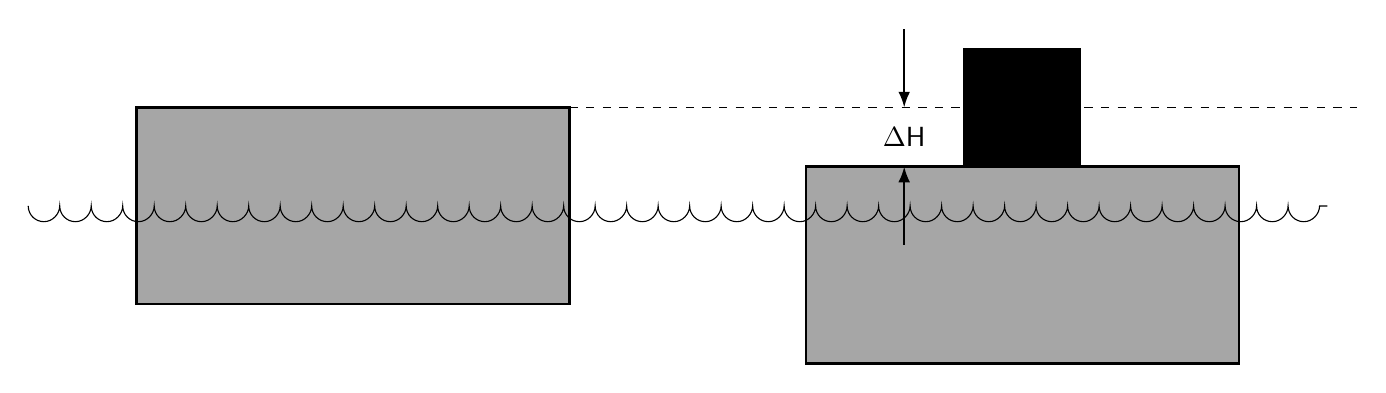
\begin{tikzpicture}[font=\sffamily, decoration={bumps, amplitude=-0.2cm, segment length=0.8cm}]
	\def\W{5.5}
	\def\H{2.5}
	\def\dist{8.5}
	\def\delH{0.75}
	\def\L{1.5}


	\draw[thick, fill=gray!70!white]	(-0.5*\W,-0.5*\H) rectangle ++(\W,\H);
	\fill[black]	(\dist-0.5*\L,+0.5*\H-\delH) rectangle ++(\L,\L);
	\draw[thick, fill=gray!70!white]	(-0.5*\W+\dist,-0.5*\H-\delH) rectangle ++(\W,\H);
	
	\draw[dashed]	(0.5*\W,0.5*\H) --++ (right:10);
	\draw[thick, \figArrow-]	(\dist-1.5,0.5*\H) --++ (up:1);
	\node[align=center]		at (\dist-1.5,0.5*\H-0.5*\delH) {$\Delta$H};
	\draw[thick, \figArrow-]	(\dist-1.5,0.5*\H-\delH) --++ (down:1);
	
	\draw[decorate]	(-0.75*\W,0) --++ (right:3*\W);
\end{tikzpicture}







%%%%%%%%	CHAPTER 10
%%%%%%%%	DOPPLER EFFECT
\begin{tikzpicture}[font=\sffamily\Large]
	\def\T{0}
	\def\A{8}
	\def\B{14}
	\def\H{2.5}
	\coordinate (circles) at (2.25,2.75);
	
	%train track
	\draw[thick]	(-4,0) --++ (right:20);
	
	%wave fronts
	\foreach \x in {1,...,4} {
		\def\start{70}
		\def\stop{-30}
		\draw[thick] ($(circles)+({\x*cos(\start)},{\x*sin(\start)})$)	arc (\start:\stop:\x);
	}

	%pedestrians
	\node[inner sep=0pt] at (\T,1.1)	{\includegraphics[height=2.2 cm]{fig/locomotive}};
	\node[inner sep=0pt] at (\A,0)	{\includegraphics[height=\H cm]{fig/standing}};
		\node[align=center, anchor=south] at (\A,0.5*\H) {pedestrian 1};
	\node[inner sep=0pt] at (\B,0)	{\includegraphics[height=\H cm]{fig/standing}};
		\node[align=center, anchor=south] at (\B,0.5*\H) {pedestrian 2};
\end{tikzpicture}

\begin{tikzpicture}[font=\sffamily\Large]
	\def\T{4}
	\def\A{-2}
	\def\B{14}
	\def\H{2.5}
	\coordinate (circles) at (6.25,2.75);
	
	%train track
	\draw[thick]	(-4,0) --++ (right:20);
	
	%wave fronts
	\foreach \x in {1,...,4} {
		\def\start{70}
		\def\stop{-30}
		\draw[thick] ($(circles)+({\x*cos(\start)},{\x*sin(\start)})$)	arc (\start:\stop:\x);
	}

	%pedestrians
	\node[inner sep=0pt] at (\T,1.1)	{\includegraphics[height=2.2 cm]{fig/locomotive}};
	\node[inner sep=0pt] at (\A,0)	{\includegraphics[height=\H cm]{fig/standing}};
		\node[align=center, anchor=south] at (\A,0.5*\H) {pedestrian 1};
	\node[inner sep=0pt] at (\B,0)	{\includegraphics[height=\H cm]{fig/standing}};
		\node[align=center, anchor=south] at (\B,0.5*\H) {pedestrian 2};
\end{tikzpicture}







%%%%%%%%	CHAPTER 10
%%%%%%%%	SHOCKWAVES
\begin{tikzpicture}[font=\sffamily\Large]
	\coordinate (O) at (0,0);
	\def\airplane{4}
	\def\R{2}
	\def\ang{30}		% asin(R/airplane)
	\coordinate (A) at (\airplane,0);
	
	\node[inner sep=0pt] at (A)	{\includegraphics[height=0.5 cm]{fig/jet}};

	\draw[thick]	(O) circle (\R);
	\draw[dashed]	(O) node[below] {O} -- (A) node[below, yshift=-2 pt] {A};
	\draw[thick]	(-\R,{tan(\ang)*(\airplane+\R)}) -- (A);
	\draw[thick]	(-\R,{-tan(\ang)*(\airplane+\R)}) -- (A);
	\draw[dashed]	(O) -- ({90-\ang}:\R) node[above right] {B};
\end{tikzpicture}





%%%%%%%%	CHAPTER 11
%%%%%%%%	CHARGING BY INDUCTION
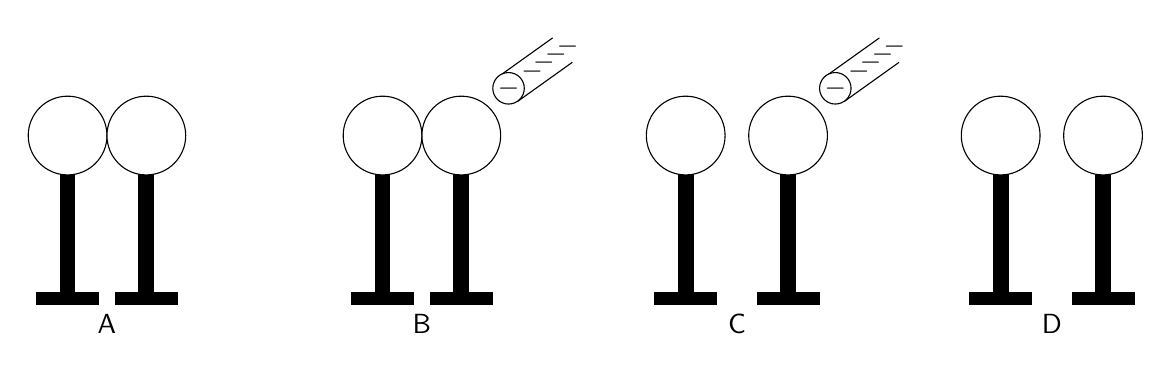
\begin{tikzpicture}[font=\sffamily]
	\tikzset	{
		sphere/.pic={
			code={       
				\fill[black]			(-0.1,0) rectangle (0.1,-2);
				\draw[fill=white]		(0,0) circle (0.5);
				\fill[black]			(-0.4,-1.99) rectangle (0.4,-2.15);
			}
		},
	}
	\tikzset	{
		rod/.pic={
			code={       
				\draw[]		(-0.14,0.14) --++ (0.7,0.5);
				\draw[]		(0.11,-0.17) --++ (0.7,0.5);
				\draw[fill=white]	(0,0) node {$-$} circle (0.2);
				\foreach \x in {1,...,4} {
					\node[]	at	({0.15+0.15*\x},{(0.15+0.15*\x)*5/7}) {$-$};
				}
			}
		},
	}
	\def\W{0.5}
	\coordinate (A) at (-\W,0);
	\coordinate (B) at (\W,0);
	\coordinate (C) at (0,-2.15);
	
	\pic[] at (A) {sphere};
	\pic[] at (B) {sphere};

	\node[align=center, anchor=north] at (C)	{A};

\begin{scope}[shift={(4,0)}]
	\def\W{0.5}
	\coordinate (A) at (-\W,0);
	\coordinate (B) at (\W,0);
	\coordinate (C) at (0,-2.15);
	
	\pic[] at ($(B)+(0.6,0.6)$) {rod};

	\pic[] at (A) {sphere};
	\pic[] at (B) {sphere};
	\node[align=center, anchor=north] at (C)	{B};	

 \end{scope}

\begin{scope}[shift={(8,0)}]
	\def\W{0.65}
	\coordinate (A) at (-\W,0);
	\coordinate (B) at (\W,0);
	\coordinate (C) at (0,-2.15);
	
	\pic[] at ($(B)+(0.6,0.6)$) {rod};

	\pic[] at (A) {sphere};
	\pic[] at (B) {sphere};
	\node[align=center, anchor=north] at (C)	{C};	

 \end{scope}

\begin{scope}[shift={(12,0)}]
	\def\W{0.65}
	\coordinate (A) at (-\W,0);
	\coordinate (B) at (\W,0);
	\coordinate (C) at (0,-2.15);
	
	\pic[] at (A) {sphere};
	\pic[] at (B) {sphere};
	\node[align=center, anchor=north] at (C)	{D};

 \end{scope}
 \end{tikzpicture}



%%%%%%%%	CHAPTER 11
%%%%%%%%	COULOMB'S LAW
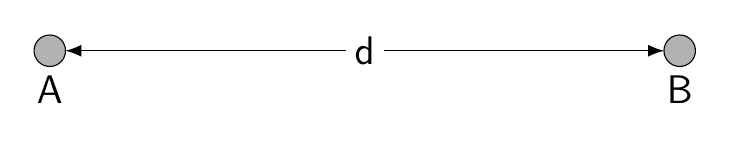
\begin{tikzpicture}[font=\sffamily\Large]
	\def\D{4}
	\def\R{0.2}
	
	\draw[fill=gray!60!white]	(-\D,0) node[below=\R cm]	{A} circle (\R);
	\draw[fill=gray!60!white]	(\D,0) node[below=\R cm]		{B} circle (\R);
	
	\draw[\figArrow-\figArrow]	(-\D+\R,0) -- (\D-\R,0) node[midway, fill=white] {d};
\end{tikzpicture}

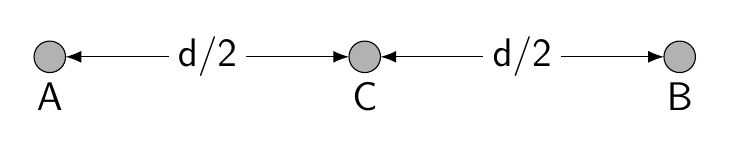
\begin{tikzpicture}[font=\sffamily\Large]
	\def\D{4}
	\def\R{0.2}
	
	\draw[fill=gray!60!white]	(-\D,0) node[below=\R cm]	{A} circle (\R);
	\draw[fill=gray!60!white]	(0,0) node[below=\R cm]		{C} circle (\R);
	\draw[fill=gray!60!white]	(\D,0) node[below=\R cm]		{B} circle (\R);
	
	\draw[\figArrow-\figArrow]	(-\D+\R,0) -- (-\R,0) node[midway, fill=white] {d/2};
	\draw[\figArrow-\figArrow]	(\R,0) -- (\D-\R,0) node[midway, fill=white] {d/2};
\end{tikzpicture}

\begin{tikzpicture}[font=\sffamily\Large]
	\def\D{4}
	\def\R{0.2}
	
	\draw[fill=gray!60!white]	(-\D,0) node[below=\R cm]	{A} circle (\R);
	\draw[fill=gray!60!white]	(-\D,\D) node[left=\R cm]	{C} circle (\R);
	\draw[fill=gray!60!white]	(\D,0) node[below=\R cm]		{B} circle (\R);
	
	\draw[\figArrow-\figArrow]	(-\D,\R) -- (-\D,\D-\R) node[midway, fill=white] {d/2};
	\draw[\figArrow-\figArrow]	(-\D+\R,0) -- (\D-\R,0) node[midway, fill=white] {d};
\end{tikzpicture}





%%%%%%%%	CHAPTER 11
%%%%%%%%	BULB AND BATTERY CIRCUITS
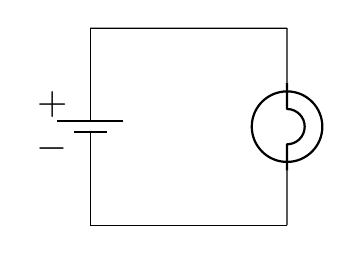
\begin{tikzpicture}[font=\sffamily\Large]
	\draw[]	(0,2.5) to [battery1, v_=~]	(0,0);
	\draw[]	(0,2.5) to [short]		(2.5,2.5);
	\draw[]	(2.5,2.5) to [bulb]		(2.5,0);
	\draw[]	(0,0) to [short]			(2.5,0);
\end{tikzpicture}
% parallel bulbs
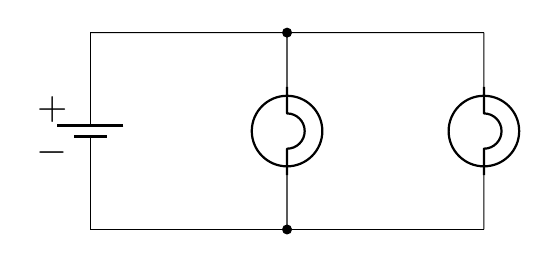
\begin{tikzpicture}[font=\sffamily\Large]
	\draw[]	(0,2.5) to [battery1, v_=~]	(0,0);
	\draw[]	(0,2.5) to [short]		(5,2.5);
	\draw[]	(2.5,2.5) to [bulb, *-*]		(2.5,0);
	\draw[]	(0,0) to [short]			(5,0);
	\draw[]	(5,2.5) to [bulb]			(5,0);
\end{tikzpicture}
% parallel batteries
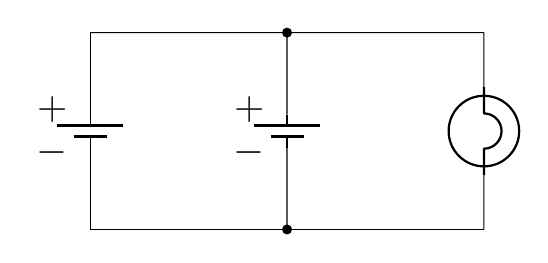
\begin{tikzpicture}[font=\sffamily\Large]
	\draw[]	(0,2.5) to [battery1, v_=~]			(0,0);
	\draw[]	(0,2.5) to [short]				(5,2.5);
	\draw[]	(2.5,2.5) to [battery1, v_=~, *-*]		(2.5,0);
	\draw[]	(0,0) to [short]					(5,0);
	\draw[]	(5,2.5) to [bulb]					(5,0);
\end{tikzpicture}
% series bulbs
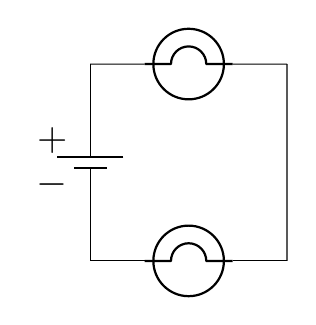
\begin{tikzpicture}[font=\sffamily\Large]
	\draw[]	(0,2.5) to [battery1, v_=~]	(0,0);
	\draw[]	(0,2.5) to [bulb]			(2.5,2.5);
	\draw[]	(2.5,2.5) to [short]		(2.5,0);
	\draw[]	(0,0) to [bulb]			(2.5,0);
\end{tikzpicture}
% series batteries
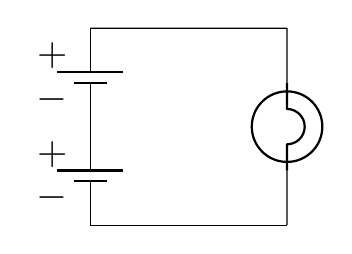
\begin{tikzpicture}[font=\sffamily\Large]
	\draw[]	(0,1.25) to [battery1, v_=~]	(0,0);
	\draw[]	(0,2.5) to [battery1, v_=~]	(0,1.25);
	\draw[]	(0,2.5) to [short]		(2.5,2.5);
	\draw[]	(2.5,2.5) to [bulb]		(2.5,0);
	\draw[]	(0,0) to [short]			(2.5,0);
\end{tikzpicture}
% series batteries with series bulbs
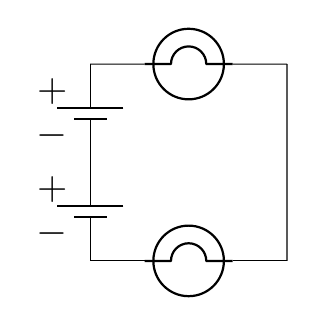
\begin{tikzpicture}[font=\sffamily\Large]
	\draw[]	(0,1.25) to [battery1, v_=~]	(0,0);
	\draw[]	(0,2.5) to [battery1, v_=~]	(0,1.25);
	\draw[]	(0,2.5) to [bulb]			(2.5,2.5);
	\draw[]	(2.5,2.5) to [short]		(2.5,0);
	\draw[]	(0,0) to [bulb]			(2.5,0);
\end{tikzpicture}







%%%%%%%%	CHAPTER 12
%%%%%%%%	TRANSFORMER
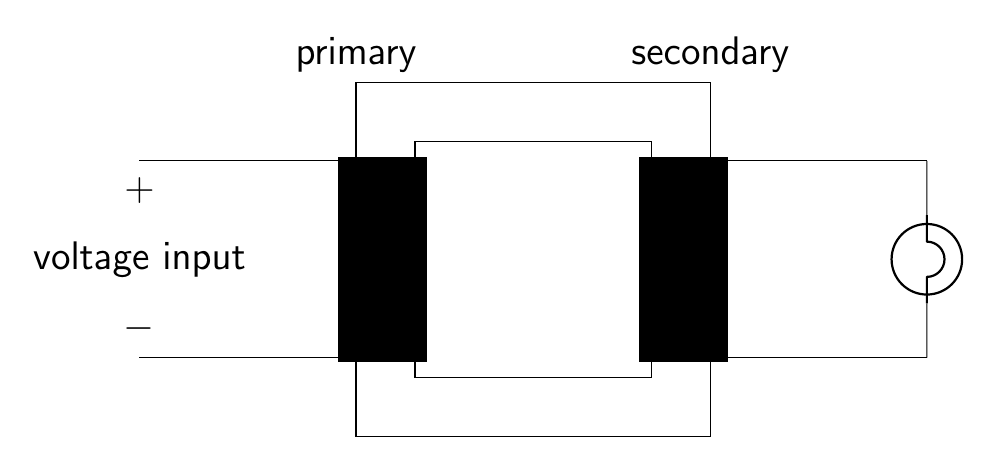
\begin{tikzpicture}[font=\sffamily\Large]
	\def\outer{4.5}
	\def\inner{3}
		\tikzset	{
		transformer/.pic={
			code={
				\draw[]		(-0.5*\outer,0.5*\outer) rectangle (0.5*\outer,-0.5*\outer);
				\draw[]		(-0.5*\inner,0.5*\inner) rectangle (0.5*\inner,-0.5*\inner);
				\fill[black]		(-0.55*\outer,1.3) rectangle (-0.45*\inner,-1.3);
				\fill[black]		(0.55*\outer,1.3) rectangle (0.45*\inner,-1.3);
			}
		},
	}
	
	\coordinate (A) at (0,0);
	
	\pic[] at (A) {transformer};
	
	\node[anchor=south, align=center] at (-0.5*\outer,0.5*\outer) {primary};
	\node[anchor=south, align=center] at (0.5*\outer,0.5*\outer) {secondary};
	
	\draw[]	(-5,1.25) to [open, v_=voltage input]	++(down:2.5);
	\draw[]	(-5,1.25) to [short] ++(right:3);
	\draw[]	(-5,-1.25) to [short] ++(right:3);

	\draw[]	(5,1.25) to [bulb]	++(down:2.5);
	\draw[]	(5,1.25) to [short] ++(left:3);
	\draw[]	(5,-1.25) to [short] ++(left:3);
\end{tikzpicture}

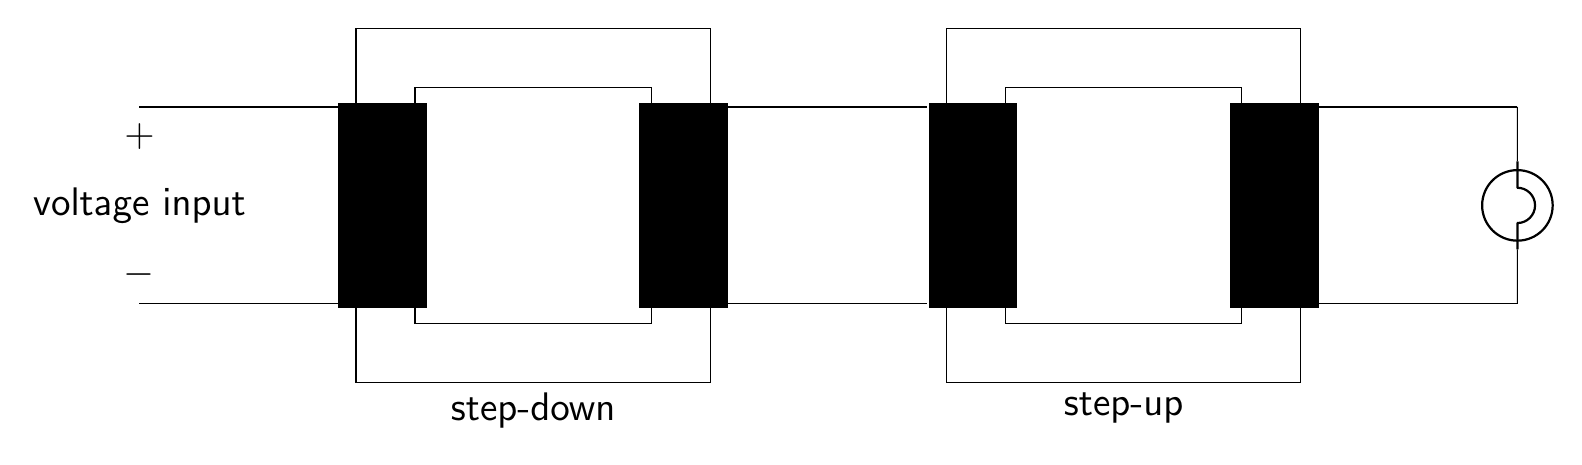
\begin{tikzpicture}[font=\sffamily\Large]
	\def\outer{4.5}
	\def\inner{3}
		\tikzset	{
		transformer/.pic={
			code={
				\draw[]		(-0.5*\outer,0.5*\outer) rectangle (0.5*\outer,-0.5*\outer);
				\draw[]		(-0.5*\inner,0.5*\inner) rectangle (0.5*\inner,-0.5*\inner);
				\fill[black]		(-0.55*\outer,1.3) rectangle (-0.45*\inner,-1.3);
				\fill[black]		(0.55*\outer,1.3) rectangle (0.45*\inner,-1.3);
			}
		},
	}
	
	\coordinate (A) at (0,0);
	\coordinate (B) at (7.5,0);
	
	\pic[] at (A) {transformer};
	\pic[] at (B) {transformer};
	
	\node[anchor=north, align=center] at (0,-0.5*\outer) {step-down};
	\node[anchor=north, align=center] at (7.5,-0.5*\outer) {step-up};
	
	\draw[]	(-5,1.25) to [open, v_=voltage input]	++(down:2.5);
	\draw[]	(-5,1.25) to [short] ++(right:3);
	\draw[]	(-5,-1.25) to [short] ++(right:3);

	\draw[]	(5,1.25) to [short] ++(left:3);
	\draw[]	(5,-1.25) to [short] ++(left:3);

	\draw[]	(12.5,1.25) to [bulb]	++(down:2.5);
	\draw[]	(12.5,1.25) to [short] ++(left:3);
	\draw[]	(12.5,-1.25) to [short] ++(left:3);
\end{tikzpicture}







%%%%%%%%	CHAPTER 13
%%%%%%%%	LAW OF REFLECTION
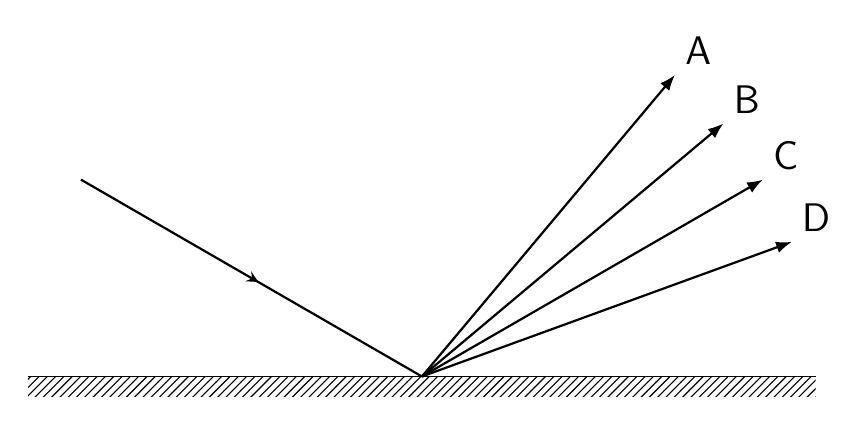
\begin{tikzpicture}[font=\sffamily\Large]
	\def\O{30}
	\def\A{130}
	\def\B{140}
	\def\C{150}
	\def\D{160}
	
	\draw[]	(-5,0) --++ (right:10);
	\fill[pattern=north east lines]	(-5,0) rectangle (5,-0.25);
	\draw[thick, arrow inside]	(-{5*cos(\O)},{5*sin(\O)}) -- (0,0);
	
	\draw[thick, -\figArrow]	(0,0) -- ({-5*cos(\A)}, {5*sin(\A)}) node[above right] {A};
	\draw[thick, -\figArrow]	(0,0) -- ({-5*cos(\B)}, {5*sin(\B)}) node[above right] {B};
	\draw[thick, -\figArrow]	(0,0) -- ({-5*cos(\C)}, {5*sin(\C)}) node[above right] {C};
	\draw[thick, -\figArrow]	(0,0) -- ({-5*cos(\D)}, {5*sin(\D)}) node[above right] {D};
\end{tikzpicture}


%%%%%%%%	CHAPTER 13
%%%%%%%%	LAW OF REFLECTION 2
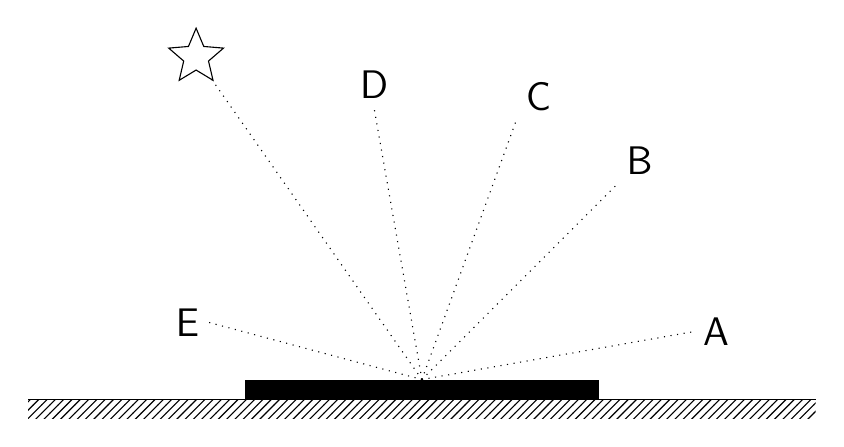
\begin{tikzpicture}[font=\sffamily\Large]
	\def\R{3.5}
	\def\Rs{5}
	\def\Re{2.8}
	\def\W{4.5}
	\def\H{0.25}
	\def\star{55}
	\def\A{170}
	\def\B{135}
	\def\C{110}
	\def\D{80}
	\def\E{15}

	
	\draw[]	(-5,-0.25) --++ (right:10);
	\fill[pattern=north east lines]	(-5,-0.25) rectangle (5,-0.5);
	\fill[black]	(-0.5*\W, -\H) rectangle (0.5*\W,0);
	
	\draw[dotted]	(0,0) -- ({-\R*cos(\A)}, {\R*sin(\A)}) node[right] {A};
	\draw[dotted]	(0,0) -- ({-\R*cos(\B)}, {\R*sin(\B)}) node[above right] {B};
	\draw[dotted]	(0,0) -- ({-\R*cos(\C)}, {\R*sin(\C)}) node[above right] {C};
	\draw[dotted]	(0,0) -- ({-\R*cos(\D)}, {\R*sin(\D)}) node[above] {D};
	\draw[dotted]	(0,0) -- ({-\Re*cos(\E)}, {\Re*sin(\E)}) node[left] {E};
	\draw[dotted]	(0,0) -- ({-\Rs*cos(\star)}, {\Rs*sin(\star)});
	
	\node [star, star point height=.2cm, minimum size=0.5cm, draw, fill=white] at ({-\Rs*cos(\star)}, {\Rs*sin(\star)}) {};
\end{tikzpicture}



%%%%%%%%	CHAPTER 13
%%%%%%%%	SNELL'S LAW
\begin{tikzpicture}[font=\sffamily\Large]
	\def\W{3}
	\def\A{50}
	\def\B{20}
	\def\C{30}
	
	\coordinate (start) at (-\W,{\W*tan(\A)});
	\coordinate (N2) at (\W,-{\W*tan(\B)});
	\coordinate (N3) at ($(N2)+(\W,-{\W*tan(\C)})$);
	
	\draw[thick, arrow inside]	(start) -- (0,0);
	\draw[thick, arrow inside]	(0,0) -- (N2);
	\draw[thick, arrow inside]	(N2) -- (N3);
	\draw[thin]				(0,5) --++ (down:10);
	\draw[thin]				(\W,5) --++ (down:10);
	\draw[dashed]			(-1,0) --++ (right:2);
	\draw[dashed]			({\W-1},-{\W*tan(\B)}) --++ (right:2);
	
	\node[align=center] at	(-0.5*\W,-4) {1};
	\node[align=center] at	(0.5*\W,-4) {2};
	\node[align=center] at	(1.5*\W,-4) {3};
\end{tikzpicture}






%%%%%%%%	CHAPTER 13
%%%%%%%%	SPEAR FISHING
\begin{tikzpicture}[font=\sffamily]
	\def\Pa{30}
	\def\Fa{60}
	\def\L{3}
	\def\P{1.5}
	\def\R{0.05}
	\coordinate (P) at (0,0);
	\coordinate (W) at (\L,-{\L*sin(\Pa)});
	\coordinate (F) at ({\L+\P},-{\L*sin(\Pa)-\P*sin(\Fa)});
	
	\node[inner sep=0pt] at (P)	{\includegraphics[height=1.5 cm]{fig/spearfish2}};
	\node[inner sep=0pt] at (F)	{\includegraphics[height=0.35 cm]{fig/fish}};

	\draw[]	($(P)+(1.06,-1)$) --++ (right:6);
	\draw[thick] decorate [decoration={random steps}]	{($(P)-(2,0.75)$) --++ (right:3) --++ (1,-3) --++ (5,-1)};
	\draw[dashed]	($(P)+(-0.2,0.5)$) -- ($(W)+(0,0.5)$);
	\draw[dashed]	($(W)+(0,0.5)$) -- (F);

	\fill[black]	($(P)+(0,1.15)$) circle (\R) node[right] {A};
	\fill[black]	($(P)-(0,0.15)$) circle (\R) node[below right, yshift=0.15 cm] {B};
	\fill[black]	($(F)+(0,0.5)$) circle (\R) node[right] {D};
	\fill[black]	($(F)-(0,0.5)$) circle (\R) node[right] {C};
\end{tikzpicture}






%%%%%%%%	CHAPTER 13
%%%%%%%%	MIRROR
\begin{tikzpicture}[font=\sffamily\Large]
	\def\H{4}
	\def\M{3}
	\def\R{3}
	\def\ang{55}
	\def\rad{0.1}

	\coordinate (you) at (-{\R*cos(\ang)},{\R*sin(\ang)});
	\coordinate (object) at (-{\R*cos(\ang)},-{\R*sin(\ang)});

	
	\draw[]	(0.25,-\H) --++ (up:2*\H);
	\fill[pattern=north east lines]	(0.25,-\H) rectangle (0.5,\H);
	\fill[black]	(0, -\M) rectangle (0.25,\M);

	\fill[black]	(you) circle (\rad) node[above] {you};
	\fill[black]	(object) circle (\rad) node[below] {object};
\end{tikzpicture}




%%%%%%%%	CHAPTER 14
%%%%%%%%	ENERGY LEVELS
\begin{tikzpicture}[font=\sffamily]
	\def\H{2}
	\def\A{0}
	\def\B{\H}
	\def\C{1.5*\H}
	\def\D{1.75*\H}
	\def\W{3}

	\draw[]	(-0.5*\W,\A) --++ (right:\W) node[right] {n=1};
	\draw[]	(-0.5*\W,\B) --++ (right:\W) node[right] {n=2};
	\draw[]	(-0.5*\W,\C) --++ (right:\W) node[right] {n=3};
	\draw[]	(-0.5*\W,\D) --++ (right:\W) node[right] {n=4};
\end{tikzpicture}
% equal energy levels
\begin{tikzpicture}[font=\sffamily]
	\def\H{0.5}
	\def\A{0}
	\def\B{\H}
	\def\C{2*\H}
	\def\D{3*\H}
	\def\W{3}

	\draw[]	(-0.5*\W,\A) --++ (right:\W) node[right] {n=1};
	\draw[]	(-0.5*\W,\B) --++ (right:\W) node[right] {n=2};
	\draw[]	(-0.5*\W,\C) --++ (right:\W) node[right] {n=3};
	\draw[]	(-0.5*\W,\D) --++ (right:\W) node[right] {n=4};
\end{tikzpicture}


















































































































































\end{document}


